% Тип документа
\documentclass[a4paper,12pt]{extarticle}

% Шрифты, кодировки, символьные таблицы, переносы
\usepackage{cmap}
\usepackage[T2A]{fontenc}
\usepackage[utf8x]{inputenc}
\usepackage[russian]{babel}
\usepackage[table]{xcolor}
% Это пакет -- хитрый пакет, он нужен но не нужен
\usepackage[mode=buildnew]{standalone}

\usepackage
	{
		% Дополнения Американского математического общества (AMS)
		amssymb,
		amsfonts,
		amsmath,
		amsthm,
		physics,
		% misccorr,
		% 
		% Графики и рисунки
		wrapfig,
		wasysym,
		graphicx,
		subcaption,
		float,
		tikz,
		tikz-3dplot,
		caption,
		csvsimple,
		color,
		booktabs,
		pgfplots,
		pgfplotstable,
		geometry,
		% 
		% Таблицы, списки
		array,
		makecell,
		multirow,
		indentfirst,
		%
		% Интегралы и прочие обозначения
		ulem,
		esint,
		esdiff,
		% 
		% Колонтитулы
		fancyhdr,
	}  

\usepackage{xcolor}
\usepackage{hyperref}

 % Цвета для гиперссылок
\definecolor{linkcolor}{HTML}{000000} % цвет ссылок
\definecolor{urlcolor}{HTML}{799B03} % цвет гиперссылок
 
\hypersetup{pdfstartview=FitH,  linkcolor=linkcolor,urlcolor=urlcolor, colorlinks=true}
% Обводка текста в TikZ
\usepackage[outline]{contour}

% Увеличенный межстрочный интервал, французские пробелы
\linespread{1.1} 
\frenchspacing 

 
\usetikzlibrary
	{
		decorations.pathreplacing,
		decorations.pathmorphing,
		patterns,
		calc,
		scopes,
		arrows,
		fadings,
		through,
		shapes.misc,
		arrows.meta,
		3d,
		quotes,
		angles,
		babel
	}

\usepgfplotslibrary{units}

% const прямым шрифтом
\newcommand\ct[1]{\text{\rmfamily\upshape #1}}
\newcommand*{\const}{\ct{const}}
\renewcommand*{\epsilon}{\varepsilon}

\usepackage[europeanresistors,americaninductors]{circuitikz}

% Style to select only points from #1 to #2 (inclusive)
\pgfplotsset{select/.style 2 args={
    x filter/.code={
        \ifnum\coordindex<#1\def\pgfmathresult{}\fi
        \ifnum\coordindex>#2\def\pgfmathresult{}\fi
    }
}}

\usepackage{array}
\usepackage{pstool}

%%%%%%%%%%%%%%%%%%%%%%%%%%%%%%%%%%%%%%%%%%%%%%%%%
\makeatletter
\newif\if@gather@prefix 
\preto\place@tag@gather{% 
  \if@gather@prefix\iftagsleft@ 
    \kern-\gdisplaywidth@ 
    \rlap{\gather@prefix}% 
    \kern\gdisplaywidth@ 
  \fi\fi 
} 
\appto\place@tag@gather{% 
  \if@gather@prefix\iftagsleft@\else 
    \kern-\displaywidth 
    \rlap{\gather@prefix}% 
    \kern\displaywidth 
  \fi\fi 
  \global\@gather@prefixfalse 
} 
\preto\place@tag{% 
  \if@gather@prefix\iftagsleft@ 
    \kern-\gdisplaywidth@ 
    \rlap{\gather@prefix}% 
    \kern\displaywidth@ 
  \fi\fi 
} 
\appto\place@tag{% 
  \if@gather@prefix\iftagsleft@\else 
    \kern-\displaywidth 
    \rlap{\gather@prefix}% 
    \kern\displaywidth 
  \fi\fi 
  \global\@gather@prefixfalse 
} 
\newcommand*{\beforetext}[1]{% 
  \ifmeasuring@\else
  \gdef\gather@prefix{#1}% 
  \global\@gather@prefixtrue 
  \fi
} 
\makeatother
%%%%%%%%%%%%%%%%%%%%%%%%%%%%%%%%%%%%%%%%%%%%%%%%%

\geometry		
	{
		left			=	2cm,
		right 			=	2cm,
		top 			=	3cm,
		bottom 			=	3cm,
		bindingoffset	=	0cm
	}

%%%%%%%%%%%%%%%%%%%%%%%%%%%%%%%%%%%%%%%%%%%%%%%%%%%%%%%%%%%%%%%%%%%%%%%%%%%%%%%

	%применим колонтитул к стилю страницы
\pagestyle{fancy} 
	%очистим "шапку" страницы
\fancyhead{} 
	%слева сверху на четных и справа на нечетных
\fancyhead[R]{\labauthors} 
	%справа сверху на четных и слева на нечетных
\fancyhead[L]{Отчёт по лабораторной работе №\labnumber} 
	%очистим "подвал" страницы
\fancyfoot{} 
	% номер страницы в нижнем колинтуле в центре
\fancyfoot[C]{\thepage} 

%%%%%%%%%%%%%%%%%%%%%%%%%%%%%%%%%%%%%%%%%%%%%%%%%%%%%%%%%%%%%%%%%%%%%%%%%%%%%%%

\renewcommand{\contentsname}{Оглавление}

\usepackage{tocloft}
% \renewcommand{\cftpartleader}{\cftdotfill{\cftdotsep}} % for parts
% \renewcommand{\cftsectiondotsep}{\cftdotsep}% Chapters should use dots in ToC
\renewcommand{\cftsecleader}{\cftdotfill{\cftdotsep}}
%\renewcommand{\cftsecleader}{\cftdotfill{\cftdotsep}} % for sections, if you really want! (It is default in report and book class (So you may not need it).
% ---------
% \newcommand{\cftchapaftersnum}{.}%
% \usepackage{titlesec}
% \titlelabel{\thetitle.\quad}
\usepackage{secdot}
\sectiondot{subsection}
\newcommand{\rot}{\operatorname{rot}}
\begin{document}

\def\labauthors{Шиков А.П.}
\def\labgroup{0420ДМР1Г}
\def\labnumber{1}
\def\labtheme{Исследование рабочих характеристик оптимального обнаружителя сложных радиолокационных сигналов.}
% \renewcommand{\vec}{\mathbf}
% \renewcommand{\phi}{\varphi}
% \renewcommand{\hat}{\widehat}

\begin{titlepage}

\begin{center}

{\small\textsc{Нижегородский государственный университет имени Н.\,И. Лобачевского}}
\vskip 1pt \hrule \vskip 3pt
{\small\textsc{Радиофизический факультет. Кафедра Радиотехники.}}

\vfill

{\Large Отчет по лабораторной работе №\labnumber\vskip 12pt\bfseries \labtheme}
	
\end{center}

\vfill
	
\begin{flushright}
	{Выполнили студенты группы \labgroup\\\ \labauthors}%\vskip 12pt Принял:\\ Менсов С.\,Н.}
\end{flushright}
	
\vfill
	
\begin{center}
	Нижний Новгород, \the\year
\end{center}

\end{titlepage}



\section{Введение}
\section{Практическая часть}
\subsection{Задание 1}
\textit{В начале отчета привести блок- схемы оптимального приемника
радиолокационного сигнала с использованием корреляторов и
согласованного фильтра, объяснить назначение их элементов. Привести
теоретические формулы для РХП в случае обнаружения известного
сигнала и сигнала со случайной фазой и амплитудой.}


Согласованный фильтр — это линейный оптимальный фильтр, построенный исходя из известных
спектральных характеристик полезного сигнала и шума. Согласованные фильтры предназначены
для выделения сигналов известной формы на фоне шумов. Под оптимальностью понимается
максимальное отношение сигнал/шум на выходе фильтра, и так как фильтр линейный форма
сигнала на выходе остается неизменной.

По определению детектор огибающей должен осуществлять измерение огибающей входного сигнала,
т.е. формировать выходной сигнал вида $u_{\text{вых}}(t) = K_{\text{дет}}A(t)$.

Пороговое устройство фильтрует сигнал в зависимости от амплитуды выходного сигнала.

устройство синхронизации запускает генерацию сигнала и интегрирование, а по
окончании этого процесса подключает к выходу интегратора пороговое
устройство.

Для обнаружителя детерминированного сигнала на фоне белого гауссова шума РХП получается только в параметрическом виде,
где параметром выступает порог обнаружения $l_0$:
\begin{equation}
    P_\text{ПО} = F\left(\frac{\ln(l_0)}{d} - d/2\right), \quad
    P_\text{ЛТ} = 1 - F\left(\frac{\ln(l_0)}{d} + d/2\right),
\end{equation}
где $F(x) = \frac{1}{\sqrt{2\pi}}\int\limits_{-\infty}^{x}\exp(-y^2/2)\dd y$ - интеграл Лапласа, $d^2 = 2 E/N_0$ - отношение
энергии сигнала к спектральной плотности мощности (СПМ) шума. 

При неизвестной фазе выражение для РХП имеет вид
\begin{equation}
    P_\text{ПО} = Q(d, \sqrt{2 \ln(1/P_\text{ЛТ})}).
\end{equation}
Здесь  $Q(v,u) = \int \limits_{u}^{\infty} x I_0 (v x) \exp \left(-\frac{x^2 + y^2}{2}\right) \dd x$ - 
фунцкия Маркума.

Если случайными являются фаза и амплитуда, выражение для РХП примет следующий вид (при условии что
распределение амплитуды имеет вид Рэлеевского):
\begin{equation}
    P_\text{ПО} = P_\text{ЛТ}^{\frac{1}{1+d^2/2}}.
\end{equation}


Для обнаружителя сигнала со случаной фазой нужно использовать два идентичных коррелятора
на которые в качестве опорных подается излучаемый сигнал и его квадратура. На выходах
корреляторов формируются действительная I и мнимая Q составляющие некоторого
аналитического сигнала.


\begin{figure}[h!]
	\centering
	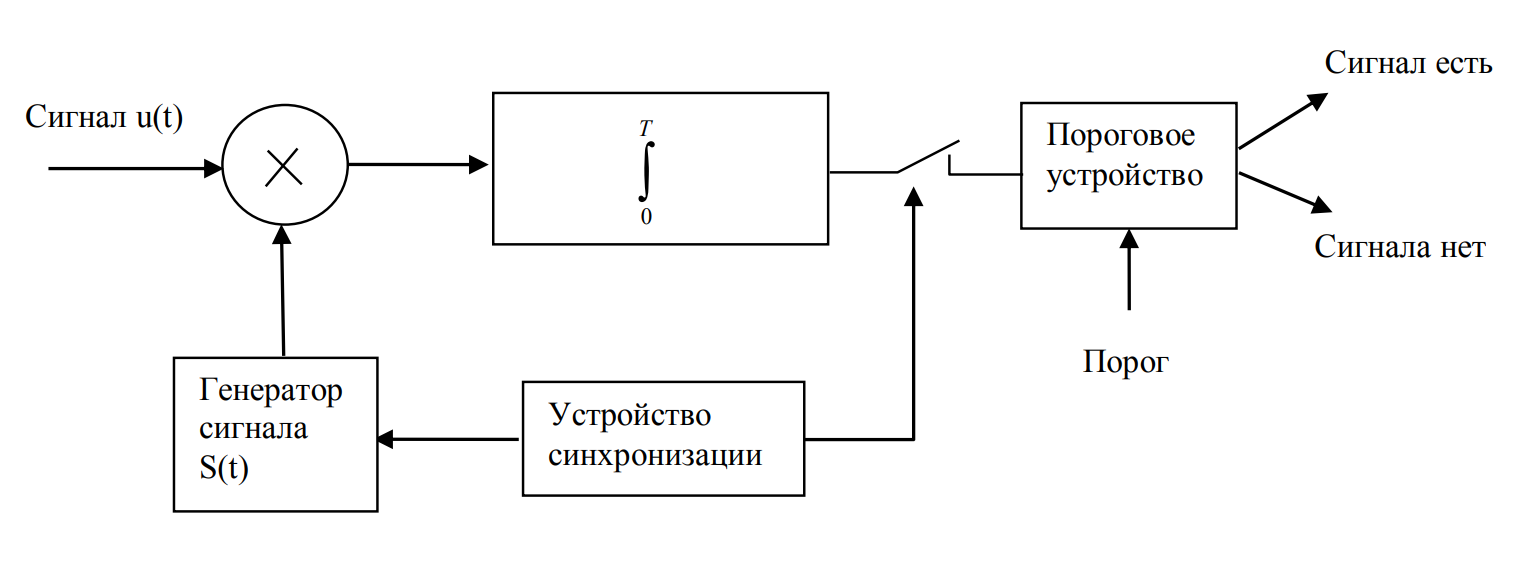
\includegraphics[width =0.8\linewidth]{imgs/scheme1.png}
	\caption{Блок-схема оптимального обнаружителя известного сигнала на фоне белого гауссова
    шума}
	\label{fig:scheme1}
\end{figure}

\begin{figure}[h!]
	\centering
	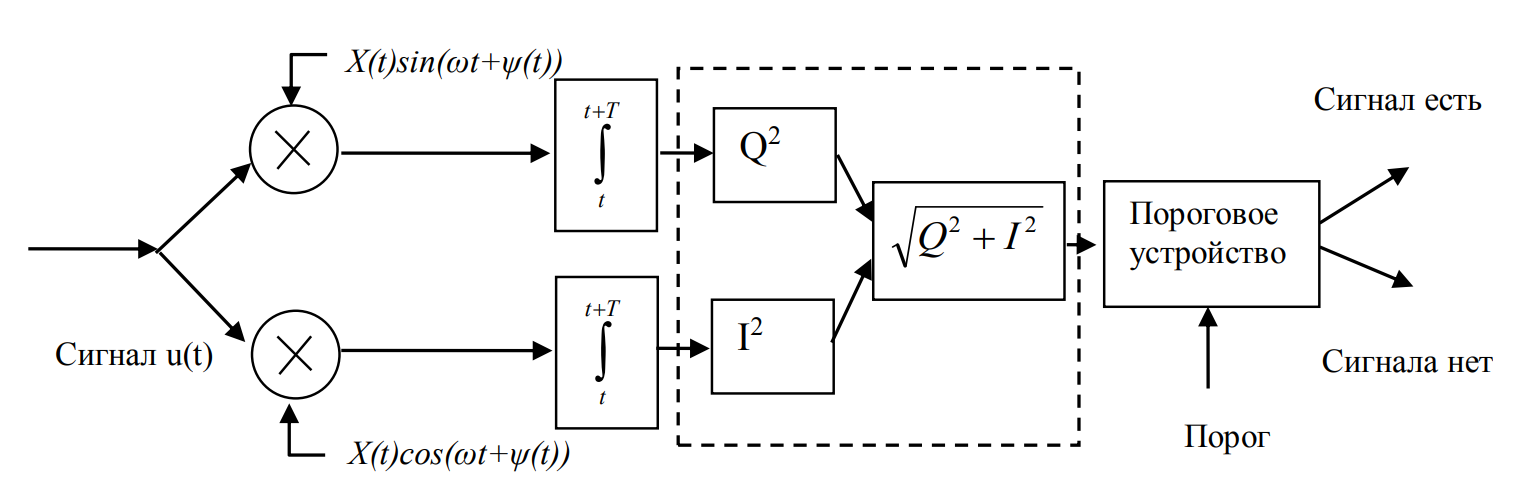
\includegraphics[width =0.8\linewidth]{imgs/scheme2.png}
	\caption{Блок-схема обнаружителя сигнала со случайной фазой и амплитудой на фоне белого
    гауссова шума с использованием двух корреляторов (устройство синхронизации на данной
    схеме отсутствует, т.к. интегрирование ведется в скользящем окне)
    }
	\label{fig:scheme2}
\end{figure}

\begin{figure}[h!]
	\centering
	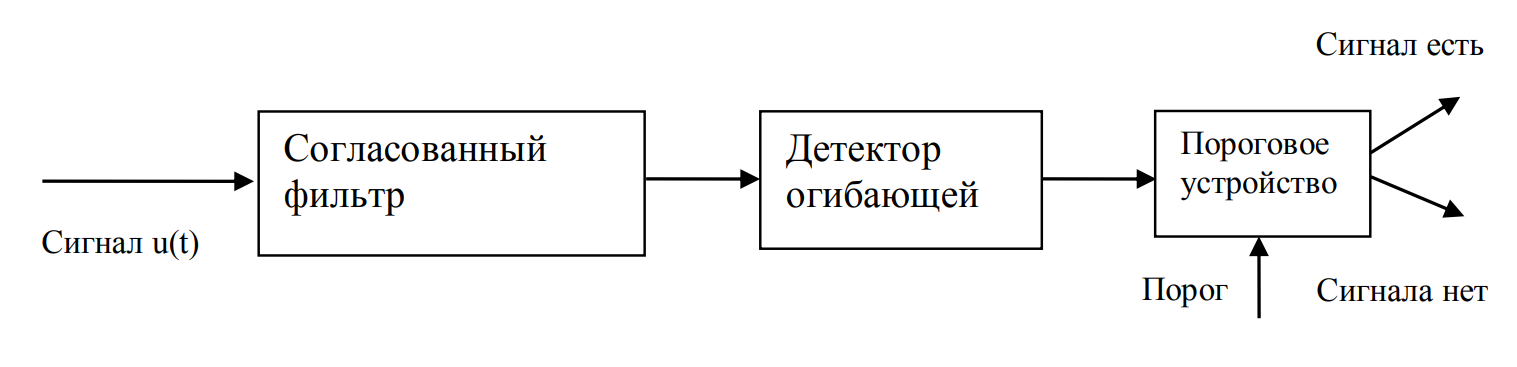
\includegraphics[width =0.8\linewidth]{imgs/scheme3.png}
	\caption{Блок-схема обнаружителя сигнала со случайной фазой и амплитудой на фоне
    белого гауссова шума с использованием согласованного фильтра и детектора огибающей}
	\label{fig:scheme3}
\end{figure}

\subsection{Задание 2}
Было проведено сравнение спектра и корреляционной функции ЛЧМ-сигнала для окна с
плоской вершиной при различных значениях разности начальной чатсоты $f_{s}$ и
конечной частот $f_{e}$. Полученные графики приведены на рис. \ref{fig:spec1}-\ref{fig:spec4}

\begin{figure}[H]
    \centering
    \begin{minipage}{0.49\linewidth}
        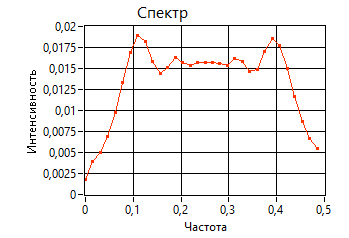
\includegraphics[width =0.9\linewidth]{imgs/spec1.png}
    \end{minipage}
    \begin{minipage}{0.49\linewidth}
        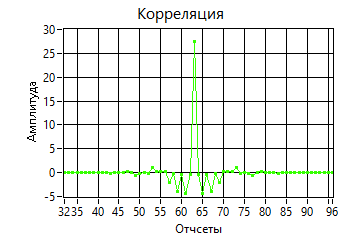
\includegraphics[width =0.9\linewidth]{imgs/corr1.png}
    \end{minipage}
	\caption{Разница частот 0.5 ($f_{s}=0, f_{e}=0.5$). Разница фаз = 0}
	\label{fig:spec1}
\end{figure}

\begin{figure}[H]
    \centering
    \begin{minipage}{0.49\linewidth}
        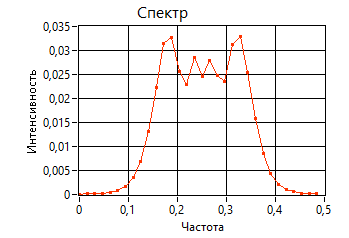
\includegraphics[width =0.9\linewidth]{imgs/spec2.png}
    \end{minipage}
    \begin{minipage}{0.49\linewidth}
        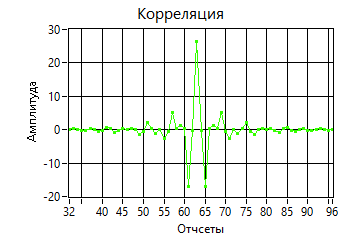
\includegraphics[width =0.9\linewidth]{imgs/corr2.png}
    \end{minipage}
	\caption{Разница частот 0.3 ($f_{s}=0.1, f_{e}=0.4$). Разница фаз = 0}
	\label{fig:spec2}
\end{figure}

\begin{figure}[H]
    \centering
    \begin{minipage}{0.49\linewidth}
        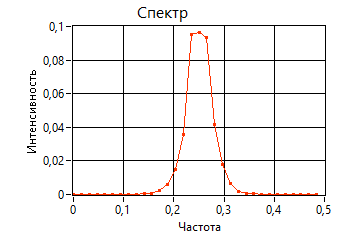
\includegraphics[width =0.9\linewidth]{imgs/spec3.png}
    \end{minipage}
    \begin{minipage}{0.49\linewidth}
        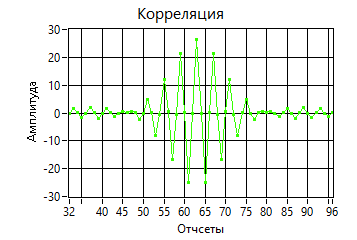
\includegraphics[width =0.9\linewidth]{imgs/corr3.png}
    \end{minipage}
	\caption{Разница частот 0.1 ($f_{s}=0.2, f_{e}=0.3$). Разница фаз = 0}
	\label{fig:spec3}
\end{figure}

\begin{figure}[H]
    \centering
    \begin{minipage}{0.49\linewidth}
        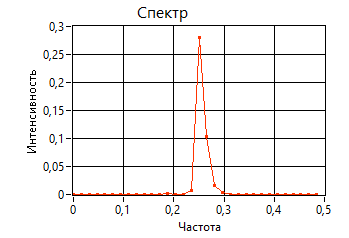
\includegraphics[width =0.9\linewidth]{imgs/spec4.png}
    \end{minipage}
    \begin{minipage}{0.49\linewidth}
        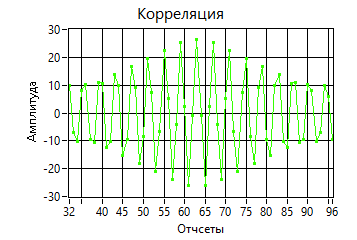
\includegraphics[width =0.9\linewidth]{imgs/corr4.png}
    \end{minipage}
	\caption{Разница частот 0.01 ($f_{s}=0.25, f_{e}=0.26$). Разница фаз = 0}
	\label{fig:spec4}
\end{figure}

Из полученных результатов видно, что при уменьшении разницы между начальной
и конечной частотой ширина корреляционной функции увеличивается, ширина спектра уменьшается,
а значение базы сигнала уменьшается.

Очевидно, что при  изменении частотной полосы ЛЧМ-сигнала его спектр
пропорционально увеличивается. Исследуемый сигнал является стационарным в
широком смысле случайным процессом, а значит его спектр связан с корреляционной
функцией обратным преобразованием Фурье

\begin{equation}
    K(\tau) = \int\limits_{-\infty}^{\infty} S(\omega) \exp{+j\omega\tau} \dd{\omega}
\end{equation}

А для пары преобразований Фурье мы можем написать соотношение неопределенности
в виде:
\begin{equation}
    \Delta \tau  \Delta \omega \geq 2\pi, \text{ где}
\end{equation} 

$\Delta \omega$ -- характерная ширина спектра, $\Delta \tau$ -- характерное ширина корреляции.

Уменьшенеие ширины спектра объясняется уменьшением количества частотных компонент, использованных 
в сигнале. Таким образм, при устремлении разницы частот к нулю, вид спектра будет приближаться к $\delta$-функции.


\subsection{Задание 3}
Построить на одном графике зависимости вероятности правильного
обнаружения от вероятности ложной тревоги для трех значений
отношения сигнал/шум при известном сигнале. Сделать то же для сигнала
со случайной фазой и случайной фазой и амплитудой. 

\begin{figure}[H]
	\centering
	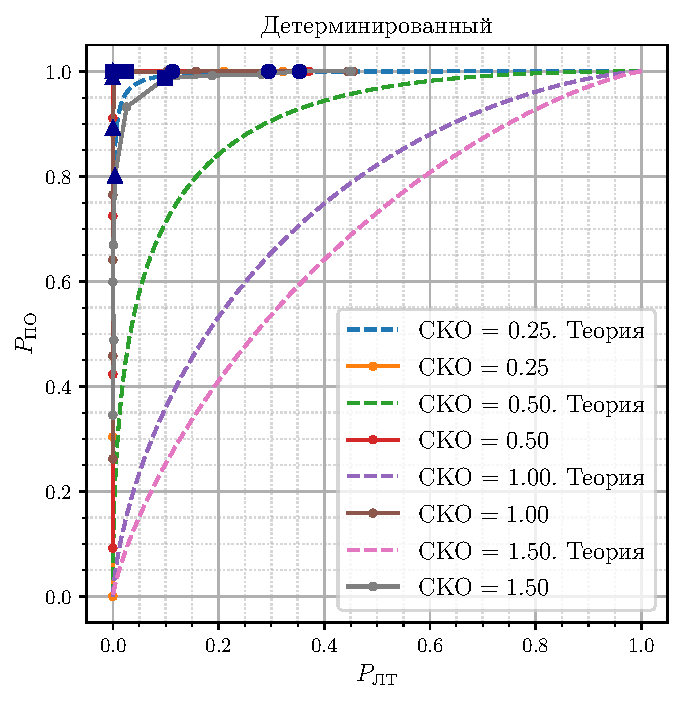
\includegraphics[width =0.5\linewidth]{data/data_determ.pdf}
	\caption{}
	\label{fig:1}
\end{figure}
\begin{figure}[H]
	\centering
	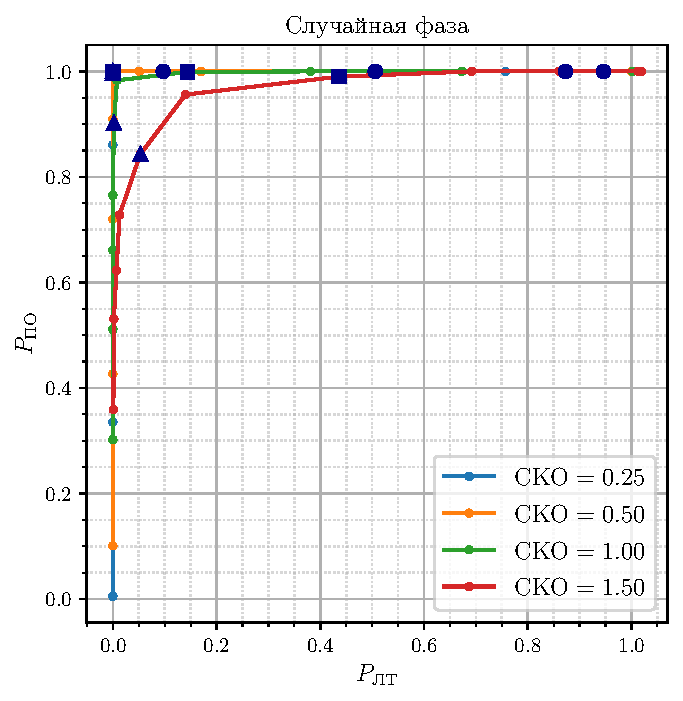
\includegraphics[width =0.5\linewidth]{data/data_phase.pdf}
	\caption{}
	\label{fig:1}
\end{figure}
\begin{figure}[H]
	\centering
	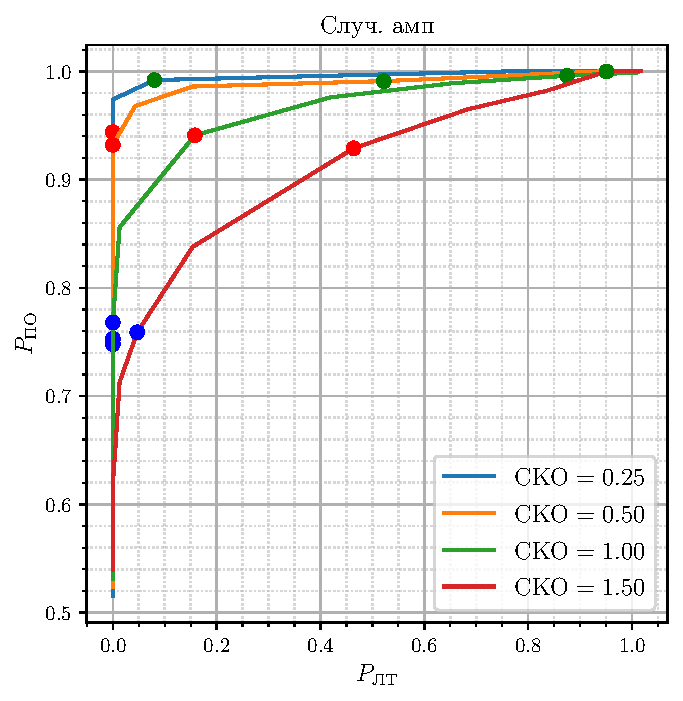
\includegraphics[width =0.5\linewidth]{data/data_amplitude.pdf}
	\caption{}
	\label{fig:1}
\end{figure}
\begin{figure}[H]
	\centering
	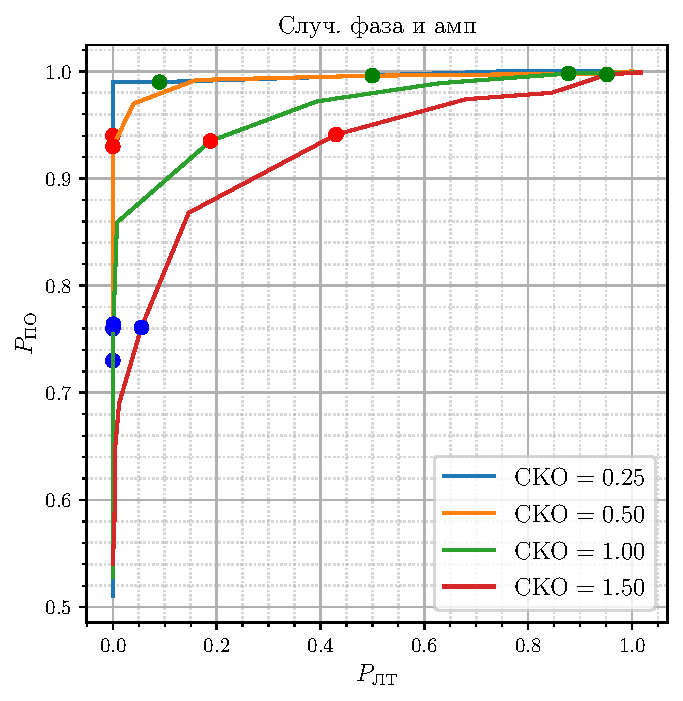
\includegraphics[width =0.5\linewidth]{data/data_phase_amplitude.pdf}
	\caption{}
	\label{fig:1}
\end{figure}

\subsection{Задание 4}
На графиках указать несколько одинаковых значений порога. Объяснить
различия между графиками. Используя формулы для РХП, сравнить
экспериментальные результаты с теоретическими.
\section{Вывод}

\end{document}
